\documentclass{beamer}

\usepackage{listings}

\usepackage{enumitem}
\setlist[enumerate]{label*=\arabic*.}

\title{Jedit Log Viewer}
\author{Troy Taillefer}
\institute{Broadsoft}

\date{\today}

\begin{document}
\setbeamertemplate{bibliography item}[text]
\setbeamertemplate{frametitle continuation}{}
\lstset{
basicstyle=\tiny,
language=Java,
showstringspaces=false,
keywordstyle=\bfseries\color{green!40!black},
commentstyle=\itshape\color{purple!40!black},
stringstyle=\color{orange},
}

\frame{\titlepage}

%Forecast
% high leve description of what problem was attacked and major insight
\begin{frame}[fragile,allowframebreaks]{Introduction}
The goal of the project was to provide an excellent tool for analyzing xs logs 
for both general understanding and trouble shooting purposes. To meet this goal three
principal features were developed

\begin{enumerate}
\item Search
\item Level of Detail
\item Navigation/Discovery
\end{enumerate}
\end{frame}

% Outline not sure what goes here Toc
\begin{frame}[fragile,allowframebreaks]{Outline}
\begin{enumerate}
\item Background
\begin{enumerate}
\item Motivation
\item Related Work
\item Search
\item Level of Detail
\item Navigation/Discovery
\end{enumerate}
\item Future Work
\item Summary
\end{enumerate}
\end{frame}


%Background
% Motivation and Problem statement (1-2) Slides
\begin{frame}[fragile,allowframebreaks]{Motivation}
XS Logs are not easy to understand and 
it is painful to stare at mono color text. I wanted to have some of the same facilities available when looking at code syntax coloring, folding, navigation and search. 
\end{frame}

% Related Work 1 slide
\begin{frame}[fragile,allowframebreaks]{Related Work}

\begin{enumerate}
\item LogViewer
\item Loogle\cite{Loogle}
\item SipSpider
\item Alexandre Blais's Scripts
\end{enumerate}
\end{frame}

\begin{frame}[fragile,allowframebreaks]{Search}
Search is the quickest way to get find you want it is far more efficient then Navigation.
Search offers very little in the way of discoverability and is very unfriendly to novices. 
This project implements search using the Jedit\cite{Jedit}\cite{Ford08} standard 
text editor search facility as well use Jedit's Beanshell\cite{Beanshell} macro 
facility to store and hot key pre-canned useful searches. 
\end{frame}

\begin{frame}[fragile,allowframebreaks]{Example Beanshell Search Macro}
\begin{lstlisting}
SearchAndReplace.setSearchString("^INVITE sip:");
SearchAndReplace.setAutoWrapAround(true);
SearchAndReplace.setRegexp(true);
SearchAndReplace.setSearchFileSet(new CurrentBufferSet());
SearchAndReplace.find(view);
\end{lstlisting}
\end{frame}

\begin{frame}[fragile,allowframebreaks]{Level of Detail}
XS logs contain a lot of information, the relevance of this information varies 
quite a bit therefore it is useful to easily hide irrelevant information. 
The three principle ways this is achieved in this project are 

\begin{enumerate}
\item Folding via a Jedit Plugin I wrote called XsLogFolder\cite{XSLogFolder} 
\item Filtering Table of Contents using Jedit's Sidekick Plugin
\item Filtering the XS logs removing unwanted information through scripts or programs
\end{enumerate}
\end{frame}

\begin{frame}[fragile,allowframebreaks]{Navigation/Discovery}
Navigation can be thought of as the way to find things when you are not sure 
what you are looking for. It also provides a high level view and context in which you orient yourself. This project implements this feature in the following ways.

\begin{enumerate}
\item Jedit's Syntax highlighting of the xs log to draw attention to important information
\item Jedit's Sidekick plugin to generate a Table of Contents
\item Java programs\cite{XsLogToPlant} \cite{XsEventsToPlant} to convert xs log into Plantuml\cite{Plantuml} diagrams with line location hyperlinks
\item A Jedit Plugin that I wrote BatikDockable\cite{BatikDockable} an svg viewer based on Batik\cite{Batik} to view and synchronize the plantuml svg diagrams with the xs log.
\end{enumerate}

\end{frame}

\begin{frame}[fragile]{How the Visualization Works}
\begin{center}
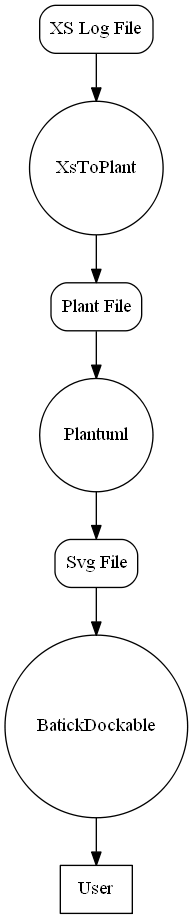
\includegraphics[height=7cm]{dattflow.png}
\end{center}
\end{frame}

\begin{frame}[fragile,allowframebreaks]{Interactive Editing}

The visualization aspect of this project has a much broader range of applicability then just viewing XS logs. As long as you can produce an
svg with link to line numbers you can reuse the technique to visualize any
text document or even interactively edit graphic languages.

Supported languages are

\begin{enumerate}
\item Plantuml\cite{Plantuml}
\item Graphviz\cite{Graphviz}
\item Tikz\cite{Tikz} 
\end{enumerate}

\end{frame}



\begin{frame}[fragile,allowframebreaks]{Future Work}
Possible future side projects include
\begin{enumerate}
\item General applicability of Beanshell to our work at Broadsoft
\item Unit testing project improve current frameworks
\end{enumerate}
\end{frame}


\begin{frame}[fragile,allowframebreaks]{Summary}
\begin{enumerate}
\item Special thanks to Jonathan Wood
\item Low development effort and rich feature set thanks to leveraging FOSS total lines of Code 475
\item Most useful to novices but hopefully interesting to experts too
\item Jedit is a great powerful editor
\item Questions ?
\item Feedback be brutally honest
\end{enumerate}
\end{frame}

\begin{frame}[allowframebreaks]{References}
\bibliographystyle{plain}
\bibliography{references}
\end{frame}

\end{document}